\documentclass[a4paper, 14pt]{article}

%\hypersetup
%{   colorlinks,
%    pdftitle={2.1.6. Journal},
%    pdfauthor={Володин Максим},
%    allcolors=[RGB]{010 090 200}
%}

\usepackage[T2A]{fontenc}
\usepackage[utf8]{inputenc}
\usepackage[english, russian]{babel}
\usepackage[top = 2cm, bottom = 2cm, left = 2cm, right = 2cm]{geometry}
\usepackage{indentfirst}
\usepackage{xcolor}
\usepackage{hyperref}
\usepackage{graphicx}
\usepackage{gensymb}
\usepackage{pgfplots}
\usepackage{amsmath, amsfonts, amssymb, amsthm, mathtools}
\usepackage{physics, multirow, float}
\usepackage{wrapfig, tabularx}
\usepackage{icomma} % Clever comma: 0,2 - number while 0, 2 - two numbers
\usepackage{tikz, standalone}
\usepackage{fancyhdr,fancybox}
\usepackage{lastpage}
\usepackage{booktabs}
\usepackage{listings}
\usepackage{lstmisc}

\graphicspath{{images/}}
\DeclareGraphicsExtensions{.pdf,.png,.jpg}

\restylefloat{table}
\usetikzlibrary{external}

\mathtoolsset{showonlyrefs = true} % Numbers will appear only where \eqref{} in the text LINKED
\pagestyle{fancy}
\fancyhf{}
% \fancyhead[R]{Показатель адиабаты}
% \fancyfoot[R]{\thepage /\pageref{LastPage}}
% \fancyhead[L]{2.1.2}

\pgfplotsset{compat=1.18}

\begin{document}

    \begin{center}
        \textbf{ОПРЕДЕЛЕНИЕ $C_P / C_V$ МЕТОДОМ ИЗОБАРИЧЕСКОГО РАСШИРЕНИЯ}
    \end{center}

    \noindent \textbf{Цель работы:} проверить применимость модели идеального газа \\
    \noindent \textbf{Задачи работы:} определение отношения $C_P / C_V$ для воздуха или углекислого газа по измерению
    давления в стеклянном сосуде \\
    \noindent \textbf{В работе используются:} стеклянный сосуд; U-образный жидкостный манометр; резиновая груша;
    газгольдер с углекислым газом.

    \addcontentsline{toc}{section}{Экспериментальная установка} \section*{Экспериментальная установка}

    Экспериментальная установка состоит из стеклянного сосуда $A$, объёмом около 20 л, снабженного краном $K_1$, и
    U-образного жидкостного манометра, измеряющего избыточное давление газа в сосуде.
    Схема установки показана на рисунке~\ref{fig:setup}

    \begin{figure}[h]
        \centering
        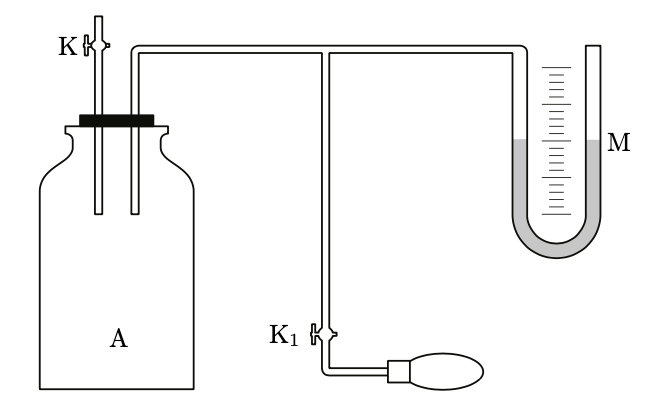
\includegraphics[width=\textwidth]{setup}
        \caption{Схема экспериментальной установки}
        \label{fig:setup}
    \end{figure}

    С помощью резиновой груши, соединённой с краном $K_1$, в сосуде создаётся заданное избыточное давление воздуха $
    P_1$.
    При этом газ оказывается перегретым

    Мысленно выделим в сосуде некоторый объём воздуха $\Delta V$.
    Будем следить за изменением его состояния.
    Вследствие теплообмена со стенками сосуда через некоторое время газ остынет до комнатной температуры $T_0$ в
    процессе изохорного охлаждения.
    При этом давление воздуха понизится до $P_0 + \Delta P_1$, где

    \begin{equation}
        \label{eq:delta1}
        \Delta P_1 = \rho g \Delta h_1
    \end{equation}

    Откроем кран $K_2$.
    За время $\Delta t$ порядка 0,5 секунд произойдёт адиабатическое расширение газа (2 $\rightarrow$ 3), и его
    температура окажется ниже комнатной.
    Далее газ будет изобарически нагреваться (процесс 3 $\rightarrow$ 4).
    Зададим время $\tau$ в течение которого кран $K_2$ остаётся открытым, таким, чтобы можно было пренебречь временем
    $\Delta t$ адиабатического расширения воздуха.
    После закрытия крана $K_2$ газ станет изохорически нагреваться до комнатной температуры (процесс 4 $\rightarrow$
    5), причём давление внутри сосуда возрастёт до $P_0 + \Delta P_2$, где

    \begin{equation}
        \label{eq:delta2}
        \Delta P_2 = \rho g \Delta h_2
    \end{equation}

    Наибольший интерес представляет исследование зависимости отношения перепадов давления $\frac{\Delta P_1}{\Delta
    P_2}$ от времени $\tau$

    С хорошей точностью мы можем считать воздух в газгольдере идеальным газом.
    Рассмотрим изобарическое расширение воздуха.
    Для этого запишем уравнение теплового баланса для изменяющейся со временем массы газа $m = \frac{P_0 V_0}{RT} \mu$:

    \[ C_P m dT = - \alpha (T - T_0) dt\]

    где $C_P$ -- удельная теплоёмкость воздуха при постоянном давлении, $\alpha$ -- положительный постоянный
    коэффициент, характеризующий теплообмен, $V_0$ -- объём газгольдера

    \[ C_P \frac{P_0 V_0}{RT} \mu dT = - \alpha (T - T_0) dt \text{ или } \frac{dT}{T(T - T_0)} = - \frac{\alpha dt}{C_P
    \frac{P_0 V_0}{R} \mu} \]

    Заметим, что
    \[ \frac{1}{T(T - T_0)} = - \frac{1}{T_0} \left( \frac{1}{T} - \frac{1}{T - T_0} \right) \]

    Тогда
    \[ \frac{1}{T_0} \left( \frac{1}{T} - \frac{1}{T - T_0} \right) dT = \frac{\alpha dt}{C_P m_0 T_0} \]

    После сокращения на $T_0$ выполним интегрирование:
    \[ \int\limits_{T_1}^{T_2} \left( \frac{1}{T} - \frac{1}{T - T_0} \right) dT = \frac{\alpha}{C_P m_0} \int\limits_{0}^{\tau} dt \text{, }  \]

    откуда
    \[ \ln \left( \frac{T_2}{T_1} \right) - \ln \left( \frac{T_2 - T_0}{T_1 - T_0} \right) = \frac{\alpha}{C_P m_0} \tau \text{ или } \ln \left( \frac{T_2}{T_1} \frac{\Delta T_1}{\Delta T_2} \right) = \frac{\alpha}{C_P m_0} \tau \]

    Наконец,
    \begin{equation}
        \label{eq:exponential_form}
        \frac{\Delta T_1}{T_1} = \frac{\Delta T_2}{T_2} \exp (\frac{\alpha}{C_P m_0} \tau)
    \end{equation}

    Для адиабатического расширения (процесс 2 $\rightarrow$ 3) справедливо соотношение $T^{\gamma} = const \cdot
    P^{\gamma - 1}$ (здесь $\gamma = \frac{C_P}{C_V}$). После взятия логарифмических производных получим:

    \[ \gamma \frac{dT}{T} = (\gamma - 1) \frac{dP}{P} \text{ или } \frac{dT}{T} = \frac{\gamma - 1}{\gamma} \frac{dP}{P} \]

    Переходя к конечным приращениям, найдём:

    \begin{equation}
        \label{eq:finite_increments}
        \frac{ \Delta T_1}{T_1} = \frac{\gamma - 1}{\gamma} \frac{\Delta P_1}{P_0}
    \end{equation}

    При изохорическом нагреве газа выполняется соотношение $\frac{P}{T} = const$.
    Возьмём от этого выражения логарифмическую производную: $\frac{dP}{P} = \frac{dT}{T}$.
    В конечных приращениях

    \begin{equation}
        \label{eq:logarithmic_quotients}
        \frac{\Delta T_2}{T_2} = \frac{\Delta P_2}{P_0}
    \end{equation}

    После подстановки~\eqref{eq:finite_increments} и~\eqref{eq:logarithmic_quotients} в~\eqref{eq:exponential_form}
    получим

    \[ \frac{\gamma - 1}{\gamma} \frac{\Delta P_1}{P_0} = \frac{\Delta P_2}{P_0} \exp \left(\frac{\alpha}{C_P m_0} \tau
    \right) \]

    Наконец, подставив в это уравнение выражения~\eqref{eq:delta1} и~\eqref{eq:delta2} получим

    \[ \frac{\gamma - 1}{\gamma} \Delta h_1 = \Delta h_2 \exp \left(\frac{\alpha}{C_P m_0} \tau\right) \text{ или }
    \frac{\Delta h_1}{\Delta h_2} = \frac{\gamma}{\gamma - 1} \exp \left(\frac{\alpha}{C_P m_0} \tau\right) \]

    Следовательно,

    \[ \ln \left(\frac{\Delta h_1}{\Delta h_2}\right) = \ln \left(\frac{\gamma}{\gamma - 1}\right) +
    \frac{\alpha}{C_P m_0} \tau \]

    Из графика зависимости $\ln \left(\frac{\Delta h_1}{\Delta h_2}\right)$ от $\tau$ определим $\gamma$

\end{document}